%%%%%%%%%%%%%%%%%%%%%%%%%%%%%%%%%%%
%This is the LaTeX ARTICLE template for RSC journals
%Copyright The Royal Society of Chemistry 2014
%%%%%%%%%%%%%%%%%%%%%%%%%%%%%%%%%%%

\documentclass[twoside,twocolumn,9pt]{article}
\usepackage{extsizes}
\usepackage[super,sort&compress,comma]{natbib} 
\usepackage[version=3]{mhchem}
\usepackage[left=1.5cm, right=1.5cm, top=1.785cm, bottom=2.0cm]{geometry}
\usepackage{balance}
\usepackage{widetext}
\usepackage{times,mathptmx}
\usepackage{sectsty}
\usepackage{graphicx} 
\usepackage{lastpage}
\usepackage[format=plain,justification=raggedright,singlelinecheck=false,font={stretch=1.125,small,sf},labelfont=bf,labelsep=space]{caption}
\usepackage{float}
\usepackage{fancyhdr}
\usepackage{fnpos}
\usepackage[english]{babel}
\usepackage{array}
\usepackage{droidsans}
\usepackage{charter}
\usepackage[T1]{fontenc}
\usepackage[usenames,dvipsnames]{xcolor}
\usepackage{setspace}
\usepackage[compact]{titlesec}
%%%Please don't disable any packages in the preamble, as this may cause the template to display incorrectly.%%%


\usepackage{epstopdf}%This line makes .eps figures into .pdf - please comment out if not required.

\definecolor{cream}{RGB}{222,217,201}

%%%MY COMMANDS
\usepackage{physics}

\newcommand*{\pd}[1]{\dfrac{\partial}{\partial #1}}
\newcommand*{\TT}{^{\mathrm{T}}}

\usepackage{color}
\newcommand*{\todo}[1]{\textbf{\textcolor{red}{#1}}}
\newcommand*{\new}[1]{\textcolor{blue}{#1}}

\begin{document}

\pagestyle{fancy}
\thispagestyle{plain}
\fancypagestyle{plain}{

%%%HEADER%%%
\fancyhead[C]{
\includegraphics[width=18.5cm]{head_foot/header_bar}}
\fancyhead[L]{\hspace{0cm}\vspace{1.5cm}
\includegraphics[height=30pt]{head_foot/journal_name}}
\fancyhead[R]{\hspace{0cm}\vspace{1.7cm}
\includegraphics[height=55pt]{head_foot/RSC_LOGO_CMYK}}
\renewcommand{\headrulewidth}{0pt}
}
%%%END OF HEADER%%%

%%%PAGE SETUP - Please do not change any commands within this section%%%
\makeFNbottom
\makeatletter
\renewcommand\LARGE{\@setfontsize\LARGE{15pt}{17}}
\renewcommand\Large{\@setfontsize\Large{12pt}{14}}
\renewcommand\large{\@setfontsize\large{10pt}{12}}
\renewcommand\footnotesize{\@setfontsize\footnotesize{7pt}{10}}
\makeatother

\renewcommand{\thefootnote}{\fnsymbol{footnote}}
\renewcommand\footnoterule{\vspace*{1pt}% 
\color{cream}\hrule width 3.5in height 0.4pt \color{black}\vspace*{5pt}} 
\setcounter{secnumdepth}{5}

\makeatletter 
\renewcommand\@biblabel[1]{#1}            
\renewcommand\@makefntext[1]% 
{\noindent\makebox[0pt][r]{\@thefnmark\,}#1}
\makeatother 
\renewcommand{\figurename}{\small{Fig.}~}
\sectionfont{\sffamily\Large}
\subsectionfont{\normalsize}
\subsubsectionfont{\bf}
\setstretch{1.125} %In particular, please do not alter this line.
\setlength{\skip\footins}{0.8cm}
\setlength{\footnotesep}{0.25cm}
\setlength{\jot}{10pt}
\titlespacing*{\section}{0pt}{4pt}{4pt}
\titlespacing*{\subsection}{0pt}{15pt}{1pt}
%%%END OF PAGE SETUP%%%

%%%FOOTER%%%
\fancyfoot{}
\fancyfoot[LO,RE]{\vspace{-7.1pt}
\includegraphics[height=9pt]{head_foot/LF}}
\fancyfoot[CO]{\vspace{-7.1pt}\hspace{13.2cm}
\includegraphics{head_foot/RF}}
\fancyfoot[CE]{\vspace{-7.2pt}\hspace{-14.2cm}
\includegraphics{head_foot/RF}}
\fancyfoot[RO]{\footnotesize{\sffamily{1--\pageref{LastPage} ~\textbar  \hspace{2pt}\thepage}}}
\fancyfoot[LE]{\footnotesize{\sffamily{\thepage~\textbar\hspace{3.45cm} 1--\pageref{LastPage}}}}
\fancyhead{}
\renewcommand{\headrulewidth}{0pt} 
\renewcommand{\footrulewidth}{0pt}
\setlength{\arrayrulewidth}{1pt}
\setlength{\columnsep}{6.5mm}
\setlength\bibsep{1pt}
%%%END OF FOOTER%%%

%%%FIGURE SETUP - please do not change any commands within this section%%%
\makeatletter 
\newlength{\figrulesep} 
\setlength{\figrulesep}{0.5\textfloatsep} 

\newcommand{\topfigrule}{\vspace*{-1pt}% 
\noindent{\color{cream}\rule[-\figrulesep]{\columnwidth}{1.5pt}} }

\newcommand{\botfigrule}{\vspace*{-2pt}% 
\noindent{\color{cream}\rule[\figrulesep]{\columnwidth}{1.5pt}} }

\newcommand{\dblfigrule}{\vspace*{-1pt}% 
\noindent{\color{cream}\rule[-\figrulesep]{\textwidth}{1.5pt}} }

\makeatother
%%%END OF FIGURE SETUP%%%

%%%TITLE, AUTHORS AND ABSTRACT%%%
\twocolumn[
  \begin{@twocolumnfalse}
\vspace{3cm}
\sffamily
\begin{tabular}{m{4.5cm} p{13.5cm} }


\includegraphics{head_foot/DOI} & \noindent\LARGE{\textbf{Identification of Nuclear Spin Isomers in full dimensionality using a quartic vibronic coupling model$^\dag$}} \\%Article title goes here instead of the text "This is the title"
\vspace{0.3cm} & \vspace{0.3cm} \\

 & \noindent\large{Sandra G\'omez,\textit{$^{a}$} Nadja Singer,\textit{$^{a}$} Graham A. Worth,$^{\ast}$\textit{$^{b}$} and Leticia Gonz\'alez$^{\ast}$\textit{$^{a}$}} \\%Author names go here instead of "Full name", etc.

\includegraphics{head_foot/dates} & \noindent\normalsize{The deactivation of 1,1-Difluoroethylene after light excitation is studied using surface hopping dynamics in presence and in absence of Rydberg states, showing that its inclusion is crucial to correctly describe the relaxation mechanism. We performed surface-hopping dynamics simulations in gas phase using aug-cc-pvdz-SA(11)-MS-CAS(2,6)PT2  and compared it to the significantly cheaper computationally aug-cc-pvdz/SA(3)-MS-CAS(2,2)PT2. Aditionally, minimal energy conical intersections (MECIs) between Rydberg and valence states and between valence and ground state were optimized using the more accurate SA(11)-MS-CAS(2,6)PT2 method. Hopping geometries were analyzed and clustered into the MECIs to unravel the deactivation pathways as well as the variation of the most relevant coordinates during the dynamics. Finally, a diabatization to asign the states to the spectroscopic notation was performed, showing that the inclusion of the Rydberg states is necessary to correctly describe the system during its internal conversion to the ground state.} \\
\end{tabular}

 \end{@twocolumnfalse} \vspace{0.6cm}

  ]
%%%END OF TITLE, AUTHORS AND ABSTRACT%%%

%%%FONT SETUP - please do not change any commands within this section
\renewcommand*\rmdefault{bch}\normalfont\upshape
\rmfamily
\section*{}
\vspace{-1cm}


%%%FOOTNOTES%%%


\footnotetext{\textit{$^{a}$~Institute for Theoretical Chemistry, Faculty of Chemistry, University of Vienna, W\"ahringerstr. 17, 1090 Vienna, Austria. E-Mail: leticia.gonzalez@univie.ac.at}}
\footnotetext{\textit{$^{b}$~Dept. of Chemistry, University College London, E-mail: g.a.worth@ucl.ac.uk}}
%Please use \dag to cite the ESI in the main text of the article.
%If you article does not have ESI please remove the the \dag symbol from the title and the footnotetext below.
\footnotetext{\dag~Electronic Supplementary Information (ESI) available: Employed LVC parameters for SO$_2$ (pdf) and research data underlying the presented figures (zip). See DOI: 10.1039/b000000x/}
%additional addresses can be cited as above using the lower-case letters, c, d, e... If all authors are from the same address, no letter is required

%%%END OF FOOTNOTES%%%

%%%MAIN TEXT%%%%
\section{Introduction}


On the quest to develop a very efficient surface hopping strategy, we present here an implementation of surface hopping dynamics using a vibronic coupling (LVC) model\cite{Koppel1984} within the SHARC (surface hopping with arbitrary couplings) molecular dynamics package.\cite{Richter2011, Mai2015, Sharc}
The approach is also suitable to compute efficiently electronic absorption spectra beyond the Condon approximation.
Vibronic coupling models are commonly used in the context of quantum dynamics, in particular within the multiconfigurational time-dependent Hartree (MCTDH) method,\cite{Beck2000} and have been shown to be a powerful method for describing ultrafast nonadiabatic processes in organic and inorganic molecules,\cite{Raab1999, Krawczyk2000, Faraji2008, Leveque2013} in transition metal complexes\cite{Worth2006, Eng2015, Fumanal2016} and at interfaces.\cite{Tamura2013}
The combination of vibronic coupling models with surface hopping offers a number of advantages to be exploited.
First, as they are computationally inexpensive, they allow for a prediction of the photophysical and photochemical behavior of a molecule without having to perform expensive on-the-fly surface hopping dynamics.
Second, as the model parameters can be computed at a high-level electronic structure method that is not feasible for the full ab initio dynamics simulations, it is possible to scrutinize the effect of a specific electronic structure level.
Third, because vibronic coupling models can be readily incorporated in quantum dynamics at the MCTDH level, it is also possible to investigate rigorously whether quantum effects going beyond the surface hopping model play a role for the system studied (see also Ref.~\citenum{Muller1997}).
%At the same time it is possible to check the influence of different degrees of freedom for performing MCTDH dynamics.

%Specifically, we present an implementation of the linear vibronic coupling (LVC) model including spin-orbit couplings in the 
%This new implementation allows the highly efficient simulation of nonadiabatic dynamics of internal conversion and ISC processes, as well as of absorption spectra beyond the Condon approximation.
%We also provide the tools that allow to determine all the required parameters from just a ground-state frequency computation and one formal surface hopping dynamics time step at the equilibrium geometry (providing the required gradients, nonadiabatic coupling vectors, and SOCs).

\begin{figure}
\centering
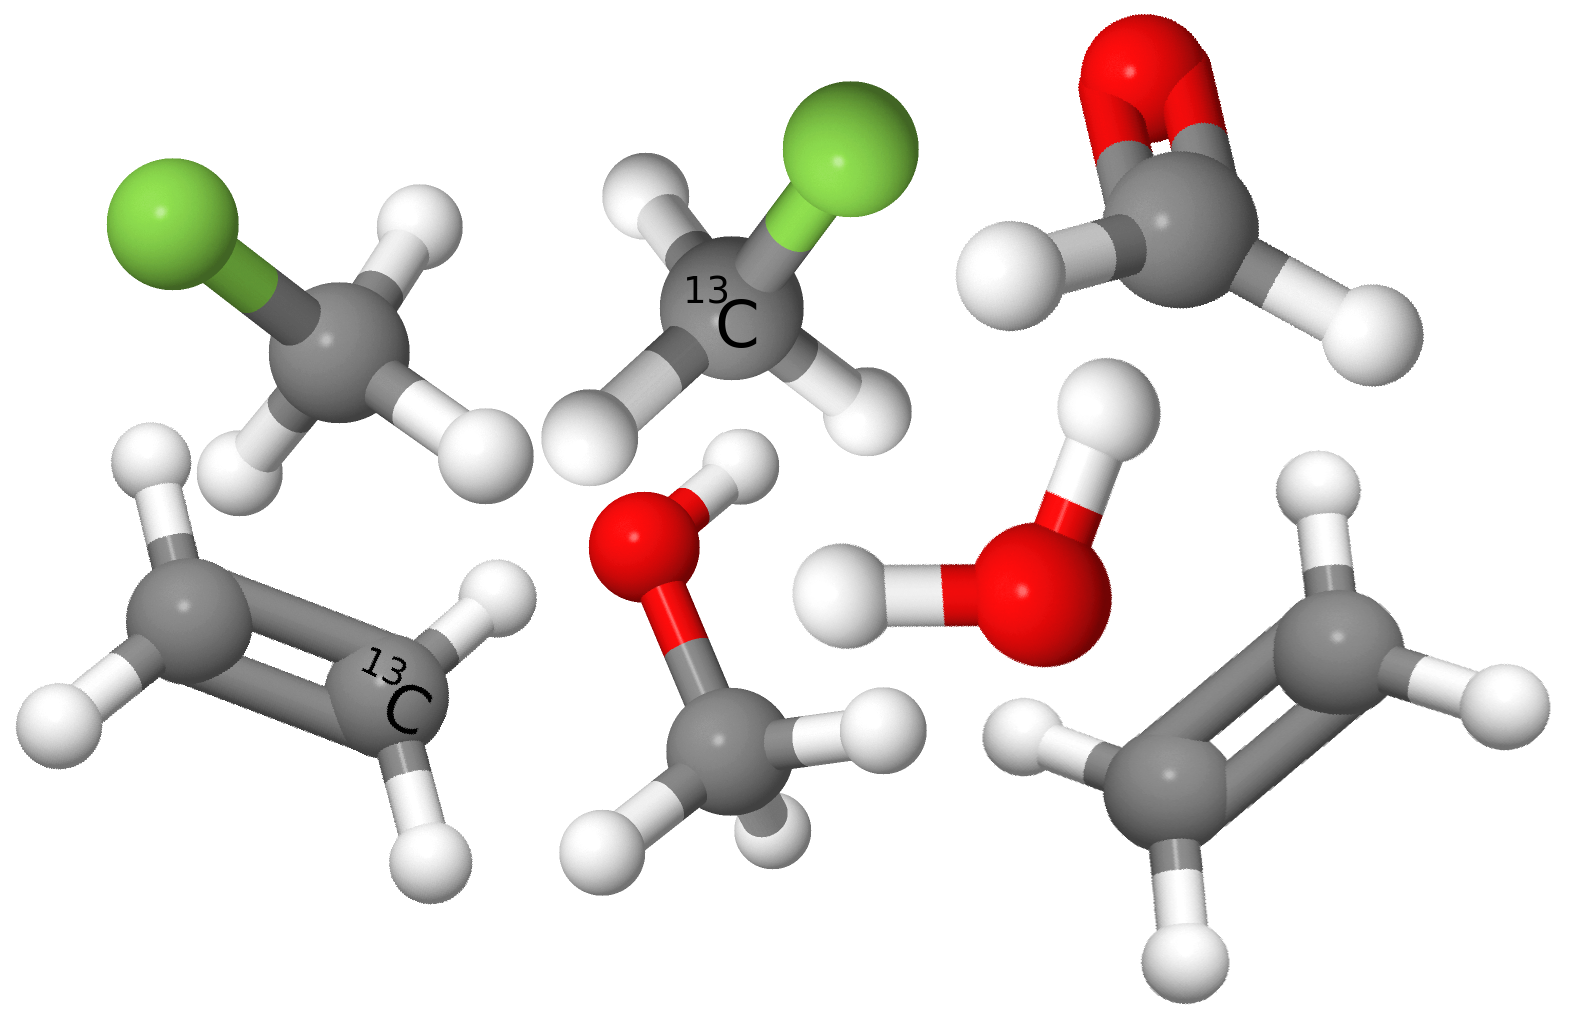
\includegraphics[width=2in]{allmolecules2}
\caption{Workflow of the SHARC/LVC method. Input quantities, intermediates and output are given in grey, blue, and red boxes, respectively. Equation numbers are shown in yellow.}
\label{fig:flow}
\end{figure}

\begin{figure}
\centering
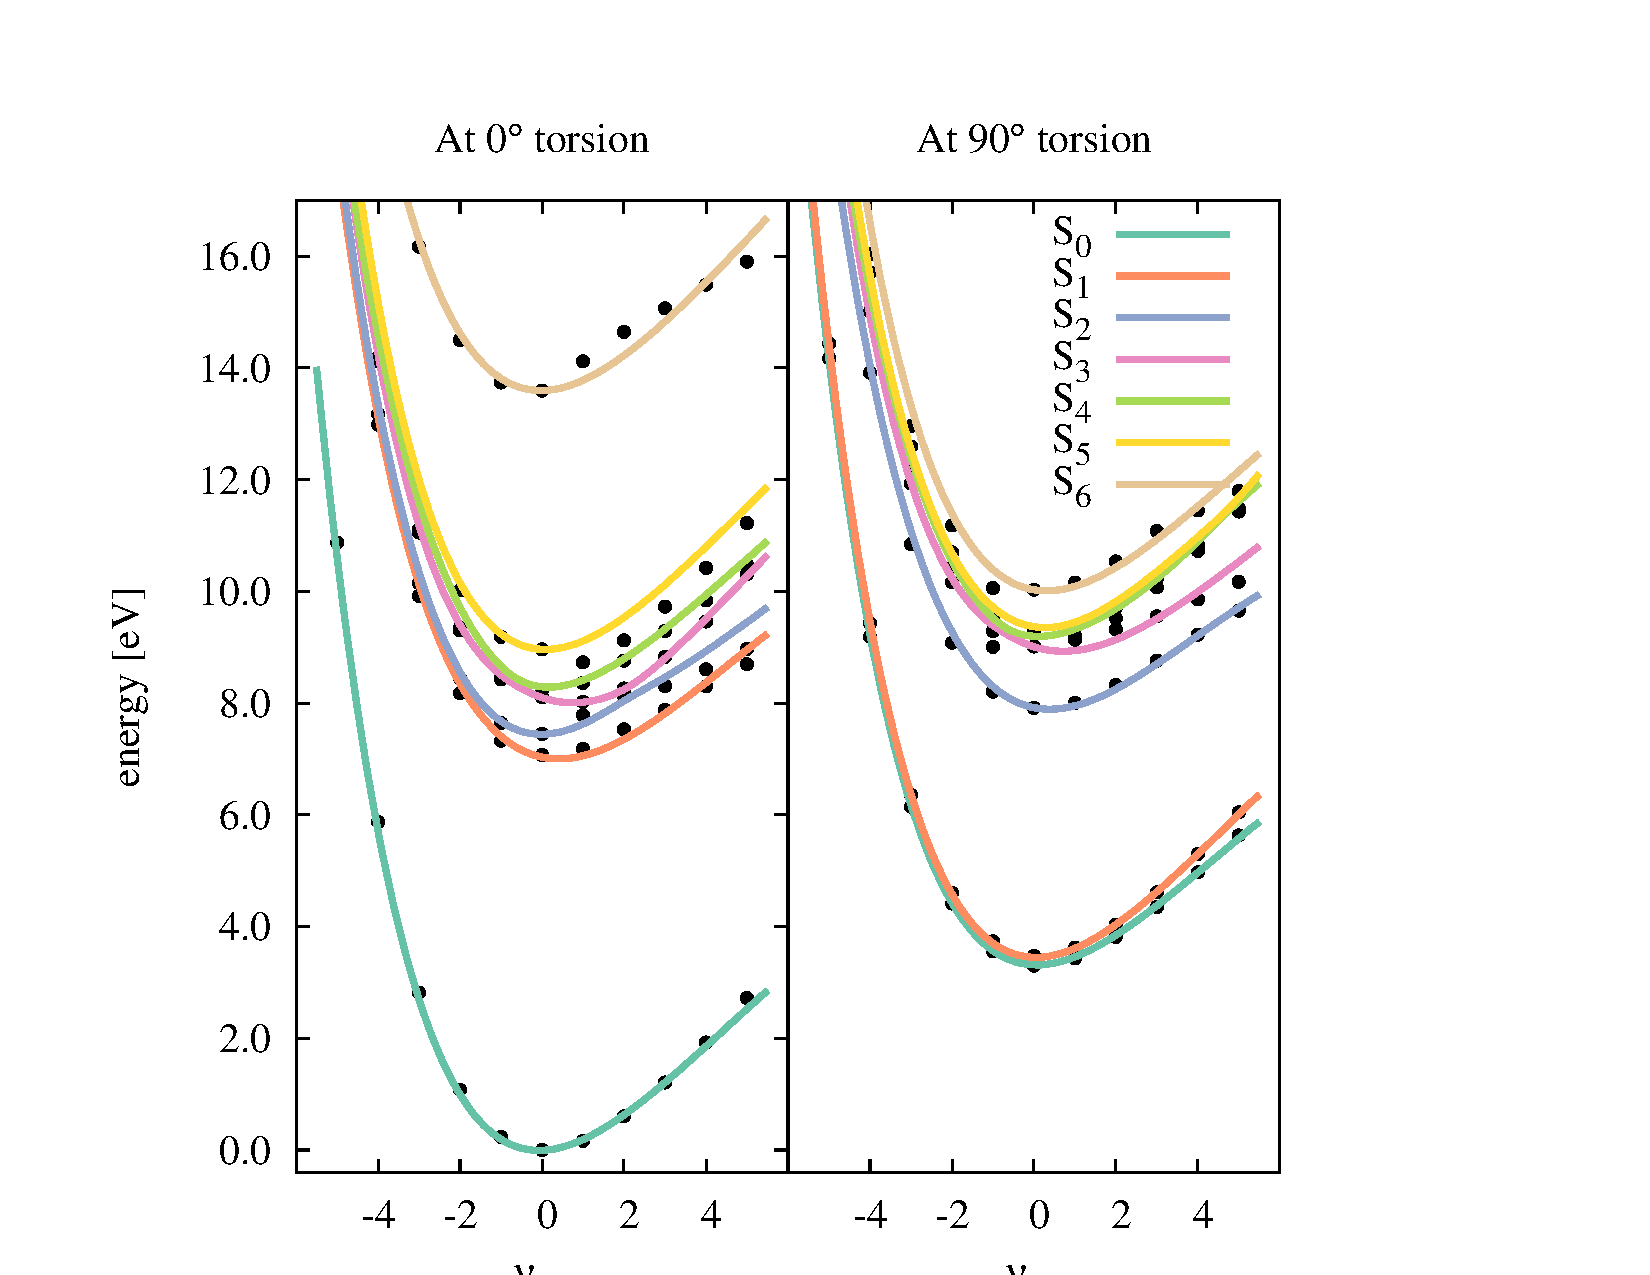
\includegraphics[width=4in]{mode11.pdf}
\caption{Workflow of the SHARC/LVC method. Input quantities, intermediates and output are given in grey, blue, and red boxes, respectively. Equation numbers are shown in yellow.}
\label{fig:flow}
\end{figure}
\begin{figure}
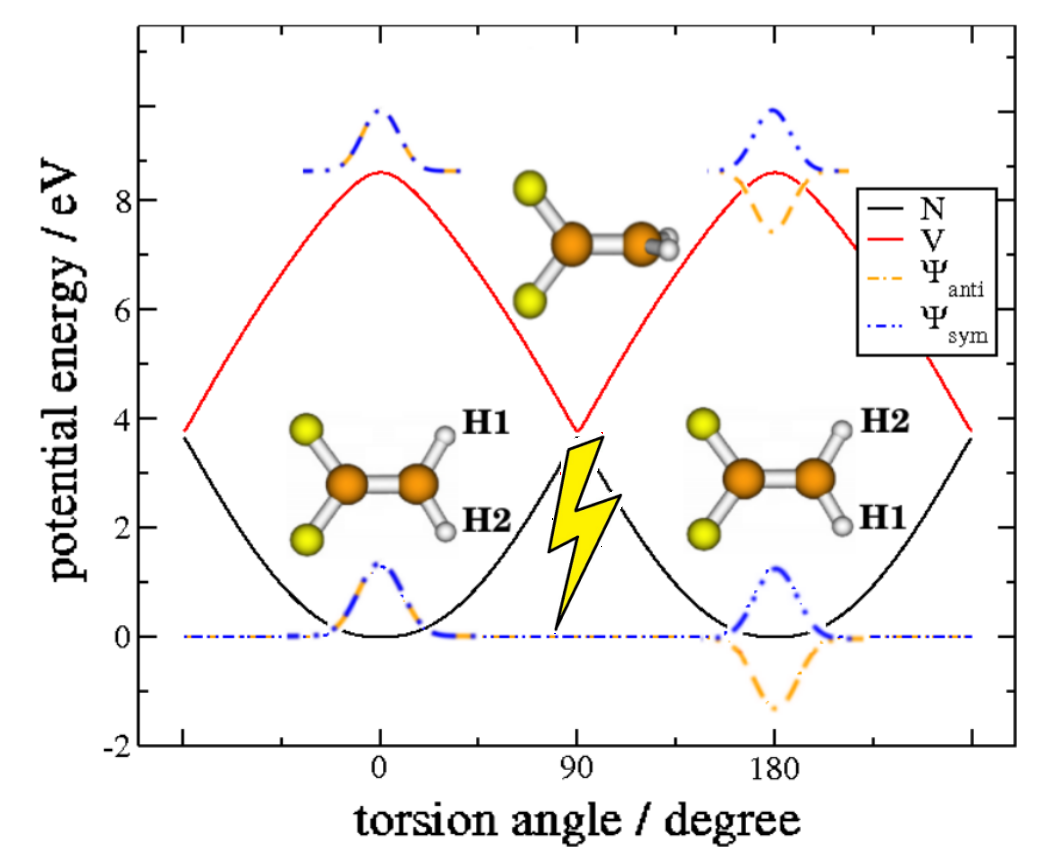
\includegraphics[width=3in]{pec1d}
\caption{Workflow of the SHARC/LVC method. Input quantities, intermediates and output are given in grey, blue, and red boxes, respectively. Equation numbers are shown in yellow.}
\label{fig:flow}
\end{figure}

Adenine undergoes non-radiative decay on a subpicosecond time scale,\cite{Ullrich2004,Evans2010,Barbatti2008,Fabiano2008,Alexandrova2010} whereas the closely related 2AP system possesses an extended excited state lifetime (> 100~ps) in gas phase\cite{Lobsiger2014} and is even fluorescent in many solvents.\cite{Guest1991,Fiebig2002} 
We will show that the present approach correctly predicts the qualitatively different behavior of these two molecules, and only requires minimal human and computational effort to do so.

\begin{figure}
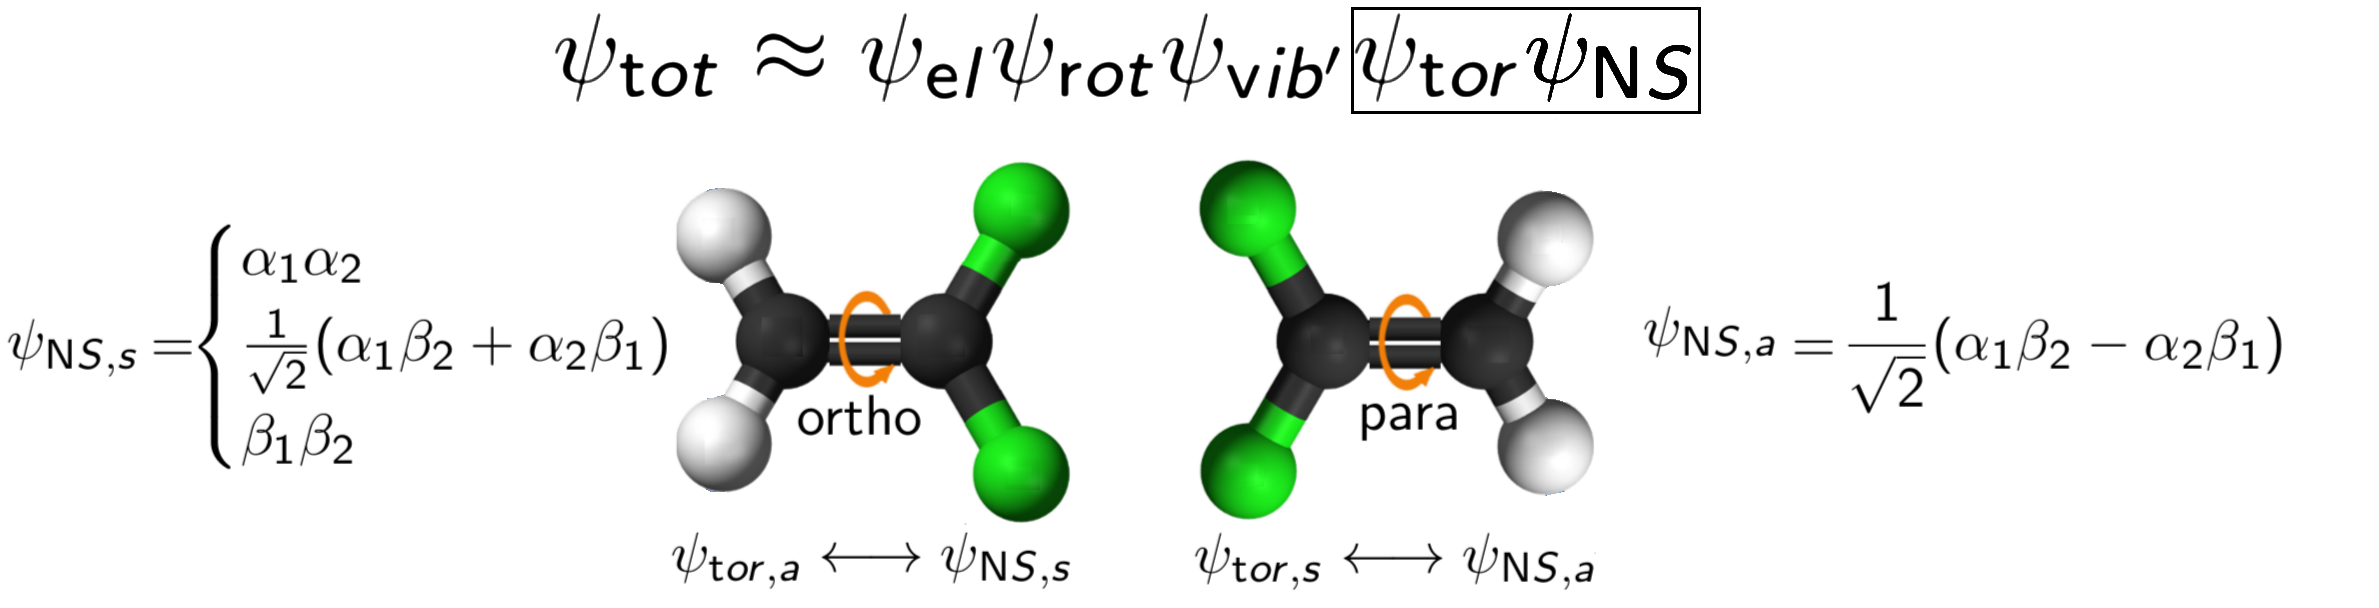
\includegraphics[width=3in]{dfe}
\caption{Workflow of the SHARC/LVC method. Input quantities, intermediates and output are given in grey, blue, and red boxes, respectively. Equation numbers are shown in yellow.}
\label{fig:flow}
\end{figure}

\section{Methods}

\begin{figure}
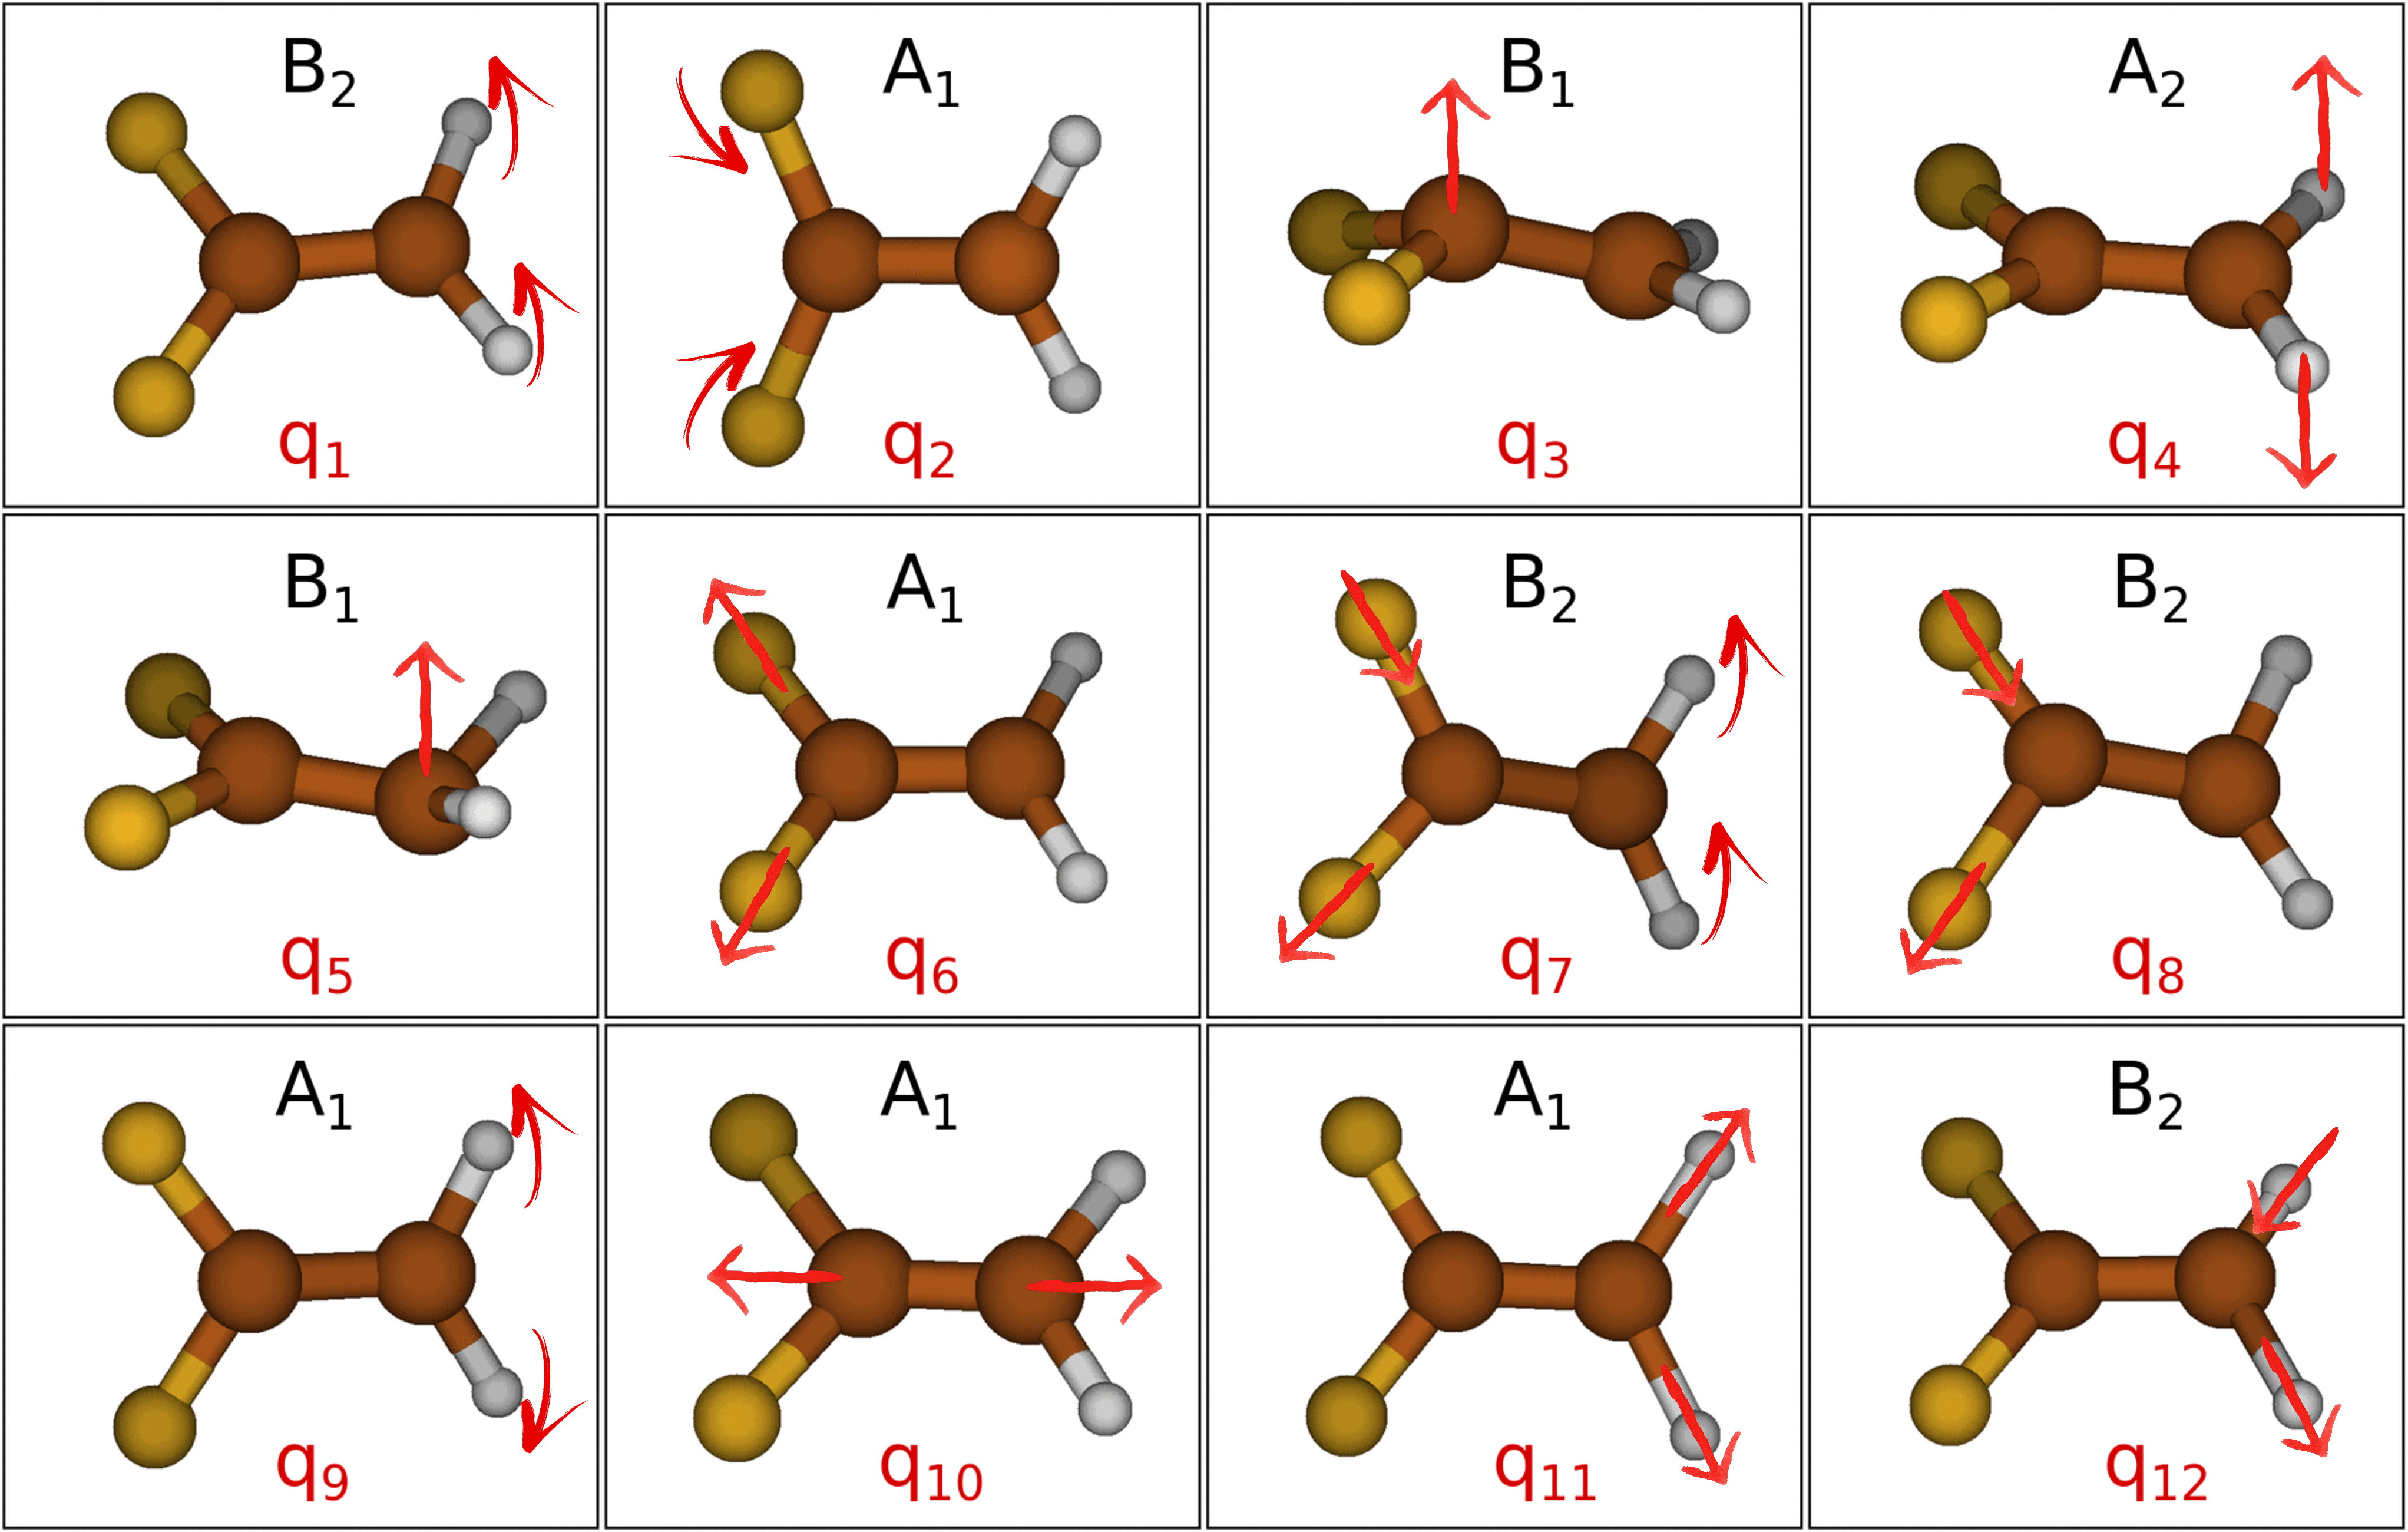
\includegraphics[width=3in]{modes}
\caption{Workflow of the SHARC/LVC method. Input quantities, intermediates and output are given in grey, blue, and red boxes, respectively. Equation numbers are shown in yellow.}
\label{fig:flow}
\end{figure}

\subsection{The Linear Vibronic Coupling Model}
In the vibronic coupling model, the molecular Coulomb Hamiltonian (MCH), i.e., the electronic Hamiltonian including Coulomb interactions but not SOC,\cite{Mai2015} is constructed in a diabatic representation as

\begin{figure}
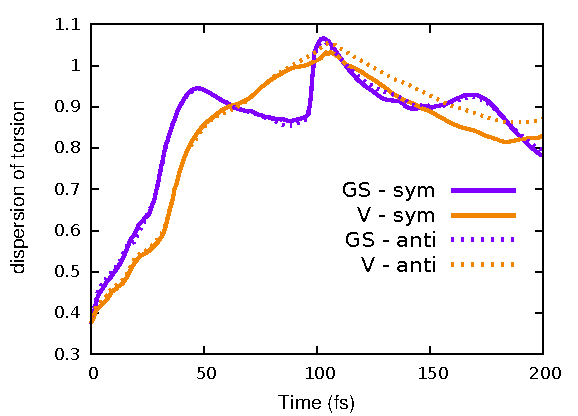
\includegraphics[width=3in]{dr4}
\caption{Workflow of the SHARC/LVC method. Input quantities, intermediates and output are given in grey, blue, and red boxes, respectively. Equation numbers are shown in yellow.}
\label{fig:flow}
\end{figure}

%
%\begin{equation}
%\hat{H}_{el} = V_0 + \sum_{m,n}\ket{\Phi_m}W_{mn}\bra{\Phi_n}
%\end{equation}
%
\begin{equation}
\label{eq:V}
\mathbf{V}=
V_0\mathbf{1}+\mathbf{W}
\end{equation}
%
where $V_0$ is the ground state potential and the $\mathbf{W}$ matrix collects the state-specific vibronic coupling terms.
In the harmonic approximation, the ground state potential is given as
%
\begin{equation}
\label{eq:V0}
V_0=
\frac{1}{2}\mathbf{r}\TT\mathbf{H}_0\mathbf{r}
\end{equation}
%
where $\mathbf{r}$ is the displacement from the reference geometry in Cartesian coordinates and $\mathbf{H}_0$ is the ground state Hessian.
To rewrite this equation, one first diagonalizes the mass-weighted Hessian
%
\begin{align}
\label{eq:Hdiag}
\sqrt{\mathbf{M}^{-1}}\mathbf{H}_0\sqrt{\mathbf{M}^{-1}} &= \mathbf{K}\Omega^2\mathbf{K}^{\rm T}\\
\Omega^2 &= \mathrm{diag}(\omega_1^2, \omega_2^2, \ldots, \omega_{3N}^2)
,
\end{align}
%
where $\mathbf{M}$ is the diagonal matrix containing the atomic masses $M_\alpha$, to obtain the normal-mode frequencies $\omega_i$ and the normal modes expressed in terms of mass-weighted coordinates (contained in the orthogonal matrix $\mathbf{K}$).
Insertion of Eq.~\eqref{eq:Hdiag} into Eq.~\eqref{eq:V0} and rearranging the terms yields
%
\begin{equation}
V_0=
\frac{\hbar}{2}\underbrace{\mathbf{r}\TT\sqrt{\mathbf{M}}\mathbf{K}\sqrt{\frac{\Omega}{\hbar}}}_{\mathbf{q}\TT}
\Omega
\underbrace{\sqrt{\frac{\Omega}{\hbar}}\mathbf{K}\TT\sqrt{\mathbf{M}}\mathbf{r}}_{\mathbf{q}}
.
\end{equation}
%
Here, the vector $\mathbf{q}=(Q_1,\ldots,Q_{3N})\TT$ represents the displacement in terms of dimensionless mass-frequency scaled normal coordinates (cf. Ref.~\citenum{Worth2004}), explicitly given as
%
\begin{equation}
\label{eq:Qi}
Q_i=\sqrt{\frac{\omega_i}{\hbar}}\sum_\alpha K_{\alpha i}\sqrt{M_\alpha}r_{\alpha}
.
\end{equation}
%
Using these coordinates, the harmonic ground state potential [Eq.~\eqref{eq:V0}] is given as
%
\begin{equation}
\label{eq:V0Qi}
V_0= \sum_i \dfrac{\hbar\omega_i}{2}Q_i^2
.
\end{equation}
%
\begin{figure}
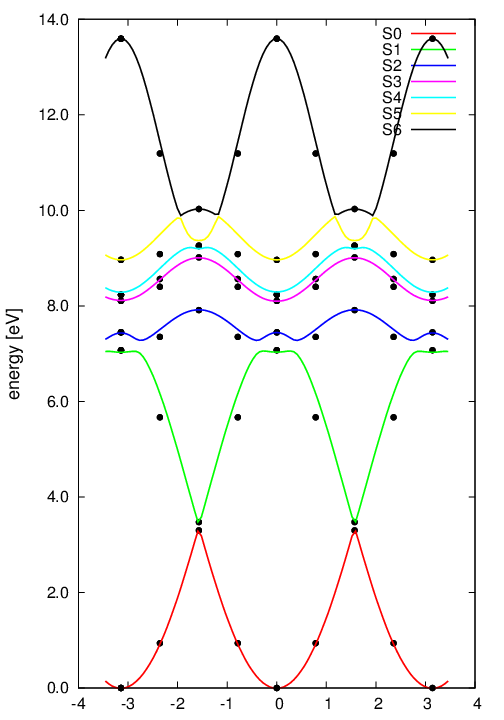
\includegraphics[width=3in]{torsion}
\caption{Workflow of the SHARC/LVC method. Input quantities, intermediates and output are given in grey, blue, and red boxes, respectively. Equation numbers are shown in yellow.}
\label{fig:flow}
\end{figure}
Within the current work, a linear vibronic coupling model (LVC) is considered, which contains the following state-specific terms in the $\mathbf{W}$ matrix.
%
\begin{align}
\label{eq:Wnn}
W_{nn}&=\epsilon_n + \sum_i\kappa_i^{(n)}Q_i\\
\label{eq:Wmn}
W_{mn}&=\sum_i\lambda_i^{(m,n)}Q_i
\end{align}
%
Here the $\epsilon_n$ are the vertical excitation energies, while the $\kappa_i^{(n)}$ and $\lambda_i^{(m,n)}$ are termed intrastate and interstate vibronic coupling constants.\cite{Koppel1984}

\subsection{Parameterization}
A new module was added to the SHARC molecular dynamics package\cite{Richter2011, Mai2015, Sharc} that allows to determine all parameters of the LVC model in a blackbox fashion, even in the case of many degrees of freedom, a high density of excited states, and the absence of symmetry.
The required input derives from a ground state frequency computation and a single-point calculation of energies, gradients, and nonadiabatic couplings at the equilibrium geometry.
%The $\omega_i$ values simply correspond to the ground state vibrational frequencies.
%The $\epsilon_n$ and $\eta_{mn}$ values are the vertical excitation energies and SOC constants at the equilibrium geometry, respectively.
Here, the intrastate vibronic coupling constants are computed as the derivative of the electronic energy $E_n$ of state $n$ with respect to a normal mode\cite{Koppel1984, Fumanal2016} computed at the reference geometry, which using Eq.~\eqref{eq:Qi} can be rearranged as
%
\begin{equation}
\label{eq:kappa}
\kappa_i^{(n)}=
\dfrac{\partial E_{n}}{\partial Q_i}
=
\sqrt{\frac{\hbar}{\omega_i}}\sum_{\alpha}\dfrac{\partial E_{n}}{\partial r_\alpha}\dfrac{K_{\alpha i}}{\sqrt{M_\alpha}}
\end{equation}
%
where $\partial E_{n}/\partial r_\alpha$ is the gradient in Cartesian coordinates.
The off-diagonal elements are defined as matrix elements of the derivative of the electronic Hamiltonian operator $\hat{H}_{el}$ with respect to a normal mode displacement\cite{Worth2004}
%
\begin{equation}
\label{eq:lambdaH}
\lambda_i^{(mn)}=
\bra{\Psi_m}\dfrac{\partial \hat{H}_{el}}{\partial Q_i}\ket{\Psi_n}=
\sqrt{\frac{\hbar}{\omega_i}}\sum_{\alpha}\bra{\Psi_m}\dfrac{\partial \hat{H}_{el}}{\partial r_\alpha}\ket{\Psi_n}\dfrac{K_{\alpha i}}{\sqrt{M_\alpha}}
\end{equation}
%
where $\Psi_m$ and $\Psi_n$ are adiabatic wavefunctions determined at the reference geometry.

Commonly, the $\lambda$ parameters are evaluated indirectly using energy-based information only, by considering either the excited state Hessian\cite{Koppel1984, Leveque2013, Fumanal2016} or by fitting the potential energy surfaces to model potentials.\cite{VCHam, Worth2004}
However, following arguments by Yarkony and coworkers,\cite{Schuurman2007}  it is possible to evaluate Eq.~\eqref{eq:lambdaH} directly and this approach is used here.
In the case of configuration interaction (CI) computations, the $\bra{\Psi_m}\partial \hat{H}_{el}/\partial r_\alpha\ket{\Psi_n}$ terms can be obtained from derivatives of the CI-matrix yielding a quantity termed $\mathbf{f}^{\mathrm{CI}}$ that is closely related to the nonadiabatic coupling vector.\cite{Lischka2004,Schuurman2007}
Similar equations have also been incorporated within coupled cluster theory.\cite{Ichino2009, Tajti2009}
In cases where nonadiabatic coupling vectors are not available, it is possible to compute the $\lambda_i^{(mn)}$ values in the same spirit through a numerical differentation using a recently described algorithm\cite{Fumanal2018JCP} based on wavefunction overlaps.\cite{OV1}
%Alternatively, it is, of course, possible to use LVC parameters obtained in any other way.

\begin{figure}
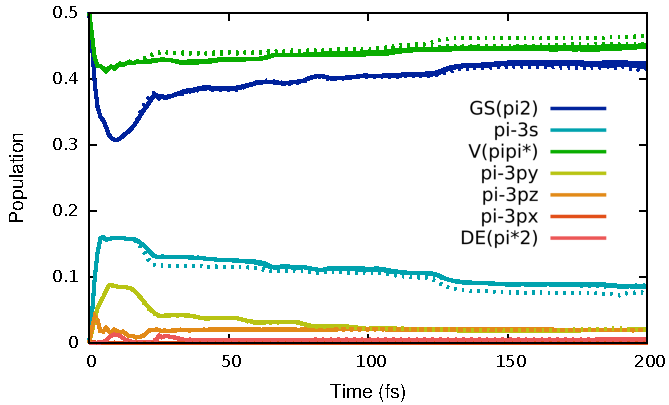
\includegraphics[width=3in]{all-pop.pdf}
\caption{Workflow of the SHARC/LVC method. Input quantities, intermediates and output are given in grey, blue, and red boxes, respectively. Equation numbers are shown in yellow.}
\label{fig:flow}
\end{figure}

\subsection{Interface to SHARC}
All quantities required by the SHARC dynamics program can be constructed from the LVC model using the workflow sketched in Figure~\ref{fig:flow}.
First, the normal mode displacements are computed from the Cartesian geometry according to Eq.~\eqref{eq:Qi}.
Then, the potential matrix $\mathbf{V}$ is computed using Eqs~\eqref{eq:V0Qi}-\eqref{eq:Wmn} and subsequently diagonalized according to
%
\begin{equation}
\mathbf{V}\mathbf{U}=\mathbf{U}\mathrm{diag}(E_1,\ldots,E_{N_{st}})
\end{equation}
%
where $\mathbf{U}$ is the diabatic-to-MCH transformation matrix and $E_n$ are the MCH energies.
Gradients and nonadiabatic couplings are computed by taking the derivatives of Eqs~\eqref{eq:V0Qi}-\eqref{eq:Wmn} with respect to normal mode displacement and subsequently transforming them to the MCH basis using the $\mathbf{U}$ matrix and to Cartesian coordinates in analogy to Eq.~\eqref{eq:Qi}.
In addition, SOCs and dipole moments can be converted from the diabatic to the MCH basis using the $\mathbf{U}$ matrix.




Wavefunction overlaps between the adiabatic wavefunctions at two successive dynamics time steps, which are needed for propagation using the local diabatization formalism,\cite{Granucci2001, locdiab} are evaluated according to
%
\begin{equation}
\mathbf{S}(t,t+\Delta t)=
\mathbf{U}(t)\TT\mathbf{U}(t+\Delta t)
.
\end{equation}

\subsection{Computational Details}
Electronic structure computations on SO$_2$ were carried out at two different levels of theory: (i) multireference configuration interaction (MR-CI)\cite{Szalay2012} including single excitations using a complete active space of 6 active electrons in 6 orbitals as reference space, and a polarized double-$\zeta$ basis set of ANO-RCC\cite{Roos2004} type [MR-CIS(6,6)/VDZP] following Ref.~\citenum{Mai2014SO2}, and (ii) MR-CI with single and double excitations using a larger (12,9) active space and a polarized triple-$\zeta$ basis set\cite{Roos2004} [MR-CISD(12,9)/VTZP].
In both cases, the orbitals were generated at the complete-active space self-consistent field level considering 12 electrons in 9 orbitals, CASSCF(12,9).
Scalar relativistic effects were taken into account by using the second-order Douglas-Kroll-Hess Hamiltonian\cite{Reiher2006} while SOC was included through atomic mean-field integrals \cite{Hess1996, Malmqvist2002} and MR-CI SOC values were computed in a perturbative fashion.\cite{Mai2014}
The $\kappa$ parameters were computed from analytical MR-CI gradients\cite{Lischka2002} and the $\lambda$ parameters were computed through derivatives of CI matrix elements.\cite{Lischka2004}
In the case of adenine and 2AP, the MR-CIS computations were performed using an active space of 10 electrons in 8 orbitals ($2\times\mathrm{n}$, $3\times\pi$, $3\times\pi^*$) and the aug-cc-pVDZ\cite{Kendall1992} basis set.
MR-CI computations were performed with the COLUMBUS program system\cite{Lischka2001, Lischka2011, Columbus_program} using integrals generated with MOLCAS\cite{Molcas_JCC} for SO$_2$ and DALTON\cite{Dalton} for Ade and 2AP.

Optical absorption spectra of SO$_2$ were computed according to a Wigner distribution of the ground state zero-point vibrational wavefunction.\cite{Dahl1988}
The surface hopping dynamics simulations on SO$_2$ were started according to the excitation windows indicated as grey rectangles in Figure~\ref{fig:spectra} (4.1-4.6~eV for MR-CIS and 3.9-4.4~eV for MR-CISD). 
4 singlet and 3 triplets states were considered in the dynamics and 200 trajectories, each, were propagated on the MR-CIS and MR-CISD potentials.
A time step length of 0.5~fs, a locally diabatic method for wavefunction propagation,\cite{Granucci2001} and  an energy-based decoherence correction ($C=0.1$~H) were used.\cite{Granucci2010}
For MCTDH,\cite{Beck2000} the vibrational ground state wavefunction was promoted to the diabatic $^1B_1$ state and the dynamics was propagated for 700 fs using 10 single particle functions per normal mode, each expressed through 32 Legendre polynomials.
UV absorption spectra were computed as the Fourier transform of the autocorrelation function obtained from the MCTDH dynamics and shifted by the zero-point energy of 0.1915~eV.

In the case of adenine the excitation window was chosen as $6.1\pm 0.1$~eV and 209 trajectories were propagated for 1000~fs considering 5 singlet states.
For 2AP the excitation window was chosen as $5.0\pm 0.1$~eV and 163 trajectories were propagated for 50~ps considering 5 singlet states.
The other set-up parameters were kept as in the previous case.
For adenine and 2AP, relaxation time constants for the $S_2\rightarrow S_1$ and $S_1\rightarrow S_0$ processes were obtained by fitting a sequential first-order kinetics model to the population data.
Errors of the time constants were obtained with the bootstrapping method,\cite{Nangia2004JCP} using 1000 bootstrapping samples for each ensemble.
Note that hese errors only describe the uncertainty due to the finite size of the trajectory ensembles, whereas they make no statement about errors due to the electronic structure and dynamics methods.

\section{Results and Discussion}
\subsection{Sulfur dioxide}
%
\begin{table}
\caption{Vertical excitation energies (eV) and oscillator strengths (given in parentheses) computed for SO$_2$ at the MR-CIS(6,6)/VDZP and MR-CISD(12,9)/VTZP levels of theory.}
\label{tab:vert}

\begin{tabular}[bth!]{ccll}
\hline
\multicolumn{2}{c}{State} & \multicolumn{1}{c}{MR-CIS} & \multicolumn{1}{c}{MR-CISD} \\
\hline
&& \\*[-0.9em]
$S_1$ & $^1B_1$ & 4.463 (0.0029) & 4.227 (0.0055) \\
$S_2$ & $^1A_2$ & 4.848 &  4.595 \\
$S_3$ & $^1B_2$ & 6.805 (0.0931) & - \\ %8.404 (0.0154) \\
$T_1$ & $^3B_1$ & 3.650 & 3.350 \\
$T_2$ & $^3B_2$ & 4.478 & 4.211  \\
$T_3$ & $^3A_2$ & 4.627 & 4.356 \\
\hline
\end{tabular}
\end{table}
%
The new method is exemplified, first, for the sulfur dioxide (SO$_2$) molecule, and its absorption spectrum as well as ultrafast intersystem crossing dynamics are investigated.
Table~\ref{tab:vert} presents the vertical excitation energies computed for the equilibrium geometry for the MR-CIS(6,6)/VDZP and MR-CISD(12,9)/VTZP levels of theory (see Computational Details).
The MR-CIS level shows that the $S_1$ state ($^1B_1$) located at 4.46~eV is the only state below 6~eV possessing oscillator strength.
The $S_2$ state ($^1A_2$) is slightly higher in energy at 4.85~eV and symmetry-forbidden.
The $S_3$ state ($^1B_2$) is well-separated and lies close to 7~eV.
The $T_1$ state ($^3B_1$) is significantly lower in energy than any singlet state while $T_2$ ($^3B_2$) and $T_3$ ($^3A_2$) are energetically close to the $S_1$ and $S_2$ states.
The ordering of the states at the MR-CISD level agrees well with that of MR-CIS but the MR-CISD values are consistently down-shifted by 0.2-0.3~eV.

\begin{figure*}[hbt!]
%\includegraphics[scale=0.9]{spectrum.pdf}
\caption{Absorption spectrum of SO$_2$ computed using six different computational protocols: Sampling of the Wigner distribution using (a) 1000 individual MR-CIS(6,6)/VDZP computations and LVC models constructed at the (b) MR-CIS(6,6)/VDZP and (e) MR-CISD(12,9)/VTZP levels; spectra computed from MCTDH dynamics using the (c) LVC(MR-CIS) and (f) LVC(MR-CISD) models.
For comparison, the LVC(MR-CIS) spectrum without interstate coupling parameters is shown in (d).
The excitation windows used for initial condition generation in the surface hopping simulations are marked as grey boxes in (a), (b), and (e).}
\label{fig:spectra}
\end{figure*}

Next, optical absorption spectra were computed for SO$_2$.
The original spectrum, computed from 1000 individual MR-CIS computations and initially reported in Ref.~\citenum{Mai2014SO2}, is shown in Figure~\ref{fig:spectra}~(a).
This spectrum is somewhat blue-shifted with respect to the experiment\cite{Golomb1962} (green line) but the spectral width is approximately reproduced.
Next, the spectrum was recomputed using the LVC model constructed at the MR-CIS level [Figure~\ref{fig:spectra}~(b)].
As explained above, all parameters for this model (see Tables S1-S4) were extracted from one single-point calculation at the equilibrium geometry.
Remarkably, the LVC spectrum reproduces the full ab initio result very well in terms of location of the peak, its width, and the amount of contribution of the $S_2$ state, with a fraction of the computational effort.
For comparison, the absorption spectrum was also computed using the MCTDH method.
This spectrum, shown in Figure~\ref{fig:spectra}~(c), exhibits a fine structure that is not obtained for the semiclassical methods, but otherwise it agrees on the position and overall broadening.
Employing the LVC model allows us to compute the spectrum also at the computationally much more expensive MR-CISD level, as presented in Figure~\ref{fig:spectra}~(e).
This spectrum is red-shifted with respect to MR-CIS by about 0.2~eV, in agreement with Table~\ref{tab:vert}, but otherwise the spectral shape is very similar.
The MCTDH spectrum computed at the LVC(MR-CISD) level is presented in Figure~\ref{fig:spectra}~(f) showing a somewhat altered fine structure when compared to the MCTDH/LVC(MR-CIS) spectrum.

An important observation regarding the spectra presented above is that the adiabatic $S_2$ state gains some intensity and contributes to the spectrum at higher energies.
This feature clearly violates the Condon approximation as the $S_2$ state is dark at the equilibrium geometry and, therefore, illustrates that the present protocol is able to compute spectra going beyond the Condon approximation.
Hence, it is interesting to compare the spectra shown above with an LVC model that ignores the interstate couplings $\lambda_i^{(mn)}$.
This corresponds to an approximation termed ``vertical gradient'',\cite{Bloino2010} meaning that the ground and excited state frequencies are the same, the oscillator strengths are constant, and only gradient information is used to construct the spectrum.
This spectrum is shown in Figure~\ref{fig:spectra}~(d) and resembles that obtained using the full LVC model [Figure~\ref{fig:spectra}~(b)] with the exception that the high-energy shoulder deriving from the adiabatic $S_2$ state cannot be reproduced.

As a next step, nonadiabatic dynamics simulations considering 4 singlet and 3 triplet states were performed for five of the computational protocols introduced in Figure~\ref{fig:spectra}.
These correspond to SHARC dynamics at the on-the-fly MR-CIS, LVC(MR-CIS), and LVC(MR-CISD) levels, as well as MCTDH simulations at the LVC(MR-CIS) and LVC(MR-CISD) levels.
Here, the difference in computational effort is noteworthy: while the 111 on-the-fly MR-CIS trajectories from Ref.~\citenum{Mai2014SO2} propagated for 700 fs require about 15000 core hours on a modern CPU, the parameterization and all 200 trajectories at the LVC(MR-CIS) level were finished in about 30 core hours.
To be able to compare results between SHARC and MCTDH we use the diabatic (spectroscopic) representation,\cite{Mai2015} i.e., we expand the time-dependent electronic wavefunctions in terms of the electronic states of the symmetric equilibrium geometry using a procedure described in more detail in Ref.~\citenum{Mai2014SO2}.
The results of the on-the-fly SHARC simulations at the MR-CIS level, orginally reported in Ref.~\citenum{Mai2014SO2}, are shown in Figure~\ref{fig:dyn}~(a).
The initial excitation goes predominantly to the $^1B_1$ state, which is the only symmetry-allowed state in the employed excitation window.
Subsequently an ultrafast transfer to the diabatic $^1A_2$ state occurs making $^1A_2$ the dominant state character already after 10~fs.
Population of the triplet states is also ultrafast and after 700~fs the total triplet population amounts to 55\%.
%$^3B_2$ is the dominant state, in agreement with Ref.~\citenum{Leveque2014}.
The LVC model [Figure~\ref{fig:dyn}~(b)] reproduces the main features of the on-the-fly simulations.
The initial inversion between the $^1B_1$ and $^1A_2$ characters occurs at exactly 10~fs.
Sub-picosecond triplet population is observed, albeit somewhat slower and after 700~fs only 38\% triplet population is reached.
The LVC method also directly allows judging the impact of quantum effects that cannot be captured by the surface hopping method.
For this purpose quantum dynamics using the MCTDH method have been carried out for the LVC(MR-CIS) model, see Figure~\ref{fig:dyn}~(c).
The results are very similar to the corresponding SHARC simulations [Figure~\ref{fig:dyn}~(b)] with the exception that stronger and more persistent oscillations between the singlet states are observed for MCTDH and that the triplet yield is somewhat lowered (only 27\% after 700~fs).

\begin{figure*}[bth!]
%\includegraphics[scale=0.9]{dyn.pdf}
\caption{Time evolution of the diabatic singlet and triplet state populations of SO$_2$  computed using five different computational protocols: (a) on-the-fly surface hopping, (b) LVC surface hopping and (c) MCDTH, all based on MR-CIS(6,6)/VDZP potentials; (d) LVC surface hopping and (e) MCTDH, both based on MR-CISD(12,9)/VTZP potentials.}
\label{fig:dyn}
\end{figure*}




Fitted time constants


\section{Conclusions}
 

\section*{Acknowledgments}
Funding from the Molim Action is gratefully acknowledged.
%%%END OF MAIN TEXT%%%



%The \balance command can be used to balance the columns on the final page if desired. It should be placed anywhere within the first column of the last page.

%\balance

%If notes are included in your references you can change the title from 'References' to 'Notes and references' using the following command:
%\renewcommand\refname{Notes and references}

%%%REFERENCES%%%
\bibliography{allrefs} %You need to replace "rsc" on this line with the name of your .bib file
\bibliographystyle{rsc} %the RSC's .bst file

\end{document}